\documentclass{article}\usepackage[]{graphicx}\usepackage[]{color}
%% maxwidth is the original width if it is less than linewidth
%% otherwise use linewidth (to make sure the graphics do not exceed the margin)
\makeatletter
\def\maxwidth{ %
  \ifdim\Gin@nat@width>\linewidth
    \linewidth
  \else
    \Gin@nat@width
  \fi
}
\makeatother

\definecolor{fgcolor}{rgb}{0.345, 0.345, 0.345}
\newcommand{\hlnum}[1]{\textcolor[rgb]{0.686,0.059,0.569}{#1}}%
\newcommand{\hlstr}[1]{\textcolor[rgb]{0.192,0.494,0.8}{#1}}%
\newcommand{\hlcom}[1]{\textcolor[rgb]{0.678,0.584,0.686}{\textit{#1}}}%
\newcommand{\hlopt}[1]{\textcolor[rgb]{0,0,0}{#1}}%
\newcommand{\hlstd}[1]{\textcolor[rgb]{0.345,0.345,0.345}{#1}}%
\newcommand{\hlkwa}[1]{\textcolor[rgb]{0.161,0.373,0.58}{\textbf{#1}}}%
\newcommand{\hlkwb}[1]{\textcolor[rgb]{0.69,0.353,0.396}{#1}}%
\newcommand{\hlkwc}[1]{\textcolor[rgb]{0.333,0.667,0.333}{#1}}%
\newcommand{\hlkwd}[1]{\textcolor[rgb]{0.737,0.353,0.396}{\textbf{#1}}}%

\usepackage{framed}
\makeatletter
\newenvironment{kframe}{%
 \def\at@end@of@kframe{}%
 \ifinner\ifhmode%
  \def\at@end@of@kframe{\end{minipage}}%
  \begin{minipage}{\columnwidth}%
 \fi\fi%
 \def\FrameCommand##1{\hskip\@totalleftmargin \hskip-\fboxsep
 \colorbox{shadecolor}{##1}\hskip-\fboxsep
     % There is no \\@totalrightmargin, so:
     \hskip-\linewidth \hskip-\@totalleftmargin \hskip\columnwidth}%
 \MakeFramed {\advance\hsize-\width
   \@totalleftmargin\z@ \linewidth\hsize
   \@setminipage}}%
 {\par\unskip\endMakeFramed%
 \at@end@of@kframe}
\makeatother

\definecolor{shadecolor}{rgb}{.97, .97, .97}
\definecolor{messagecolor}{rgb}{0, 0, 0}
\definecolor{warningcolor}{rgb}{1, 0, 1}
\definecolor{errorcolor}{rgb}{1, 0, 0}
\newenvironment{knitrout}{}{} % an empty environment to be redefined in TeX

\usepackage{alltt}
\usepackage[margin=0.5in]{geometry}
\usepackage{graphicx}
\usepackage[font={small,it}]{caption}
\usepackage{wrapfig}
\IfFileExists{upquote.sty}{\usepackage{upquote}}{}
\begin{document}



\title{Statistics Coursework}
\author{Alun Meredith}
\maketitle
\section{Reading data}
Downloaded fish.txt, data about the catch of a hypothetical fishing fleet from:\\"http://www.edshare.soton.ac.uk/view/courses/COMP6235/2015.html" on Fri Nov 20 13:48:28 2015. 

\section{Visualising Data}

\begin{figure}[h]
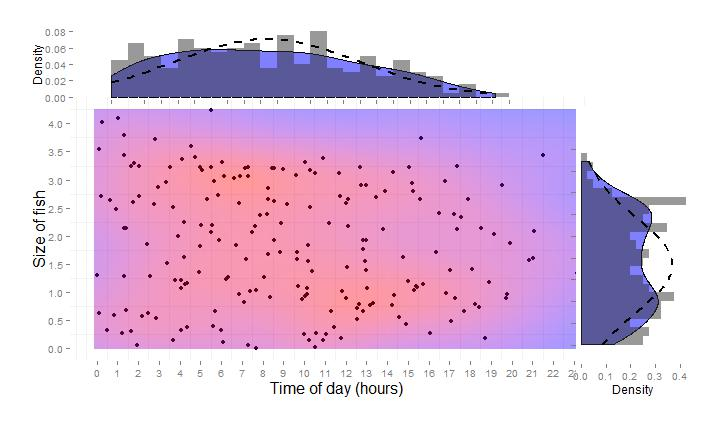
\includegraphics[width=\linewidth]{figure1.jpg}
\caption{\textbf{Bottom Left}: Scatter graph of size of fish caught vs time of day (hours), coloured background demonstrating gaussian kernel 2d density \textbf{Right}: Histogram showing distribution of size of fish caught and gaussian kernel density \textbf{Top}: Histogram showing time of day fish caught overlayed by gaussian kernel density}
\label{fig:1}
\end{figure}
% latex table generated in R 3.2.2 by xtable 1.8-0 package
% Fri Nov 20 13:47:47 2015
\begin{table}[ht]
\centering
\caption{Numeric summary statistics for Time and Size Distributions} 
\begin{tabular}{rrrrrrrrrrrr}
  \hline
 & min & Q1 & median & Q3 & max & mean & s.dev & var & skewness & kurtosis & geometric mean \\ 
  \hline
sizeSummary & 0.01 & 0.94 & 1.83 & 2.74 & 4.23 & 1.84 & 1.08 & 1.16 & 0.09 & -1.17 & 1.37 \\ 
  timesSummary & 0.01 & 4.88 & 8.95 & 13.22 & 23.16 & 9.39 & 5.66 & 32.00 & 0.25 & -0.89 & 6.79 \\ 
   \hline
\end{tabular}
\end{table}


\section{Analysing Distributions}

By looking at the above summary statistics and the density distributions in figure \ref{fig:1}, we can see some interesting features of the distributions. The time fish were caught was very broard with high standard deviation. There is some skewness which can be seen clearly in the plot. This is fairly surprising as you would expect the density at 12:01 to be approximately equal to the density at 11:59 in a cyclical manner. This suggests that an effect such as the data being recorded on a Saturday where no fishing is done on a Sunday is occuring, but requires more domain knowledge to analyse fully.

The distribution of fish sizes (right hand density plot in figure \ref{fig:1}) shows a distribution which is visibly bimodal. The standard deviation covers 51.18\% of the data range, which is greater than the wide flat times data of 48.9, this is probably due to the bimodal distributions. Both the mean and median sits centrally between the two peaks with low skewness because the peaks are approximately symmetric and equal in size. 

\subsection{Confidence Intervals}



\begin{wrapfigure}[11]{R}{6cm}
  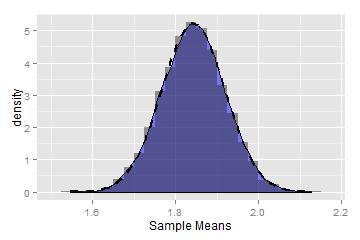
\includegraphics[width=0.9\linewidth]{figure3.jpg}
  \caption{10000 sample means taken from fish size data, blue region is density, dashed line shows normal distribution with equal mean and variance.}
  \label{fig:three}
\end{wrapfigure}

Both of the distributions are not normally distributed, the normal distributions in fig \ref{fig:1} doesn't accurately describe the observations. This introduces some complexity in producing confidence intervals. For the time caught confidence interval it is possible to closely approximate the normal distribution by transforming the data, e.g. applying an exponent of approximately 0.79 removes the bias.

In order to evaluate a confidence interval from these non-standard distributions a Bootstrapping method is used. As shown in fig.\ref{fig:three} by resampling our data and plotting the means we get a distribution that closely approximates the normal distribution via the central limit theorem. The mean of a sample distribution approximates the mean of the population it was sampled from. By calculating a confidence interval for this mean we can estimate a 95\% confidence interval for the population of:\footnote{At 3 significant figures the students t test yields the same confidence intervals, for applications where accuracy is only required at this level the students t test or normal approximation is sufficient.}

% latex table generated in R 3.2.2 by xtable 1.8-0 package
% Fri Nov 20 13:37:11 2015
\begin{table}[ht]
\centering
\begin{tabular}{rrr}
  \hline
  \hline
SizeConfidence & 1.69 & 1.99 \\ 
  TimeConfidence & 8.61 & 10.18 \\ 
   \hline
\end{tabular}
\caption{Bootstrapped confidence intervals \\ for the mean (95 percent)} 
\end{table}


\subsection{Codependency and Time intervals}






\begin{wrapfigure}[12]{ht}{6cm}
  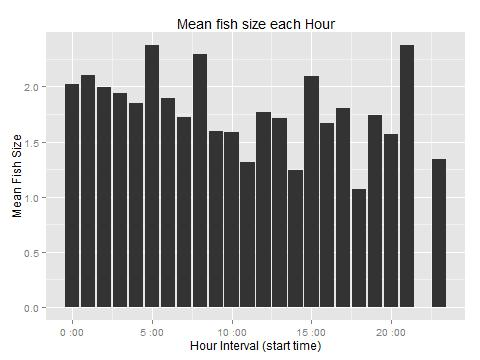
\includegraphics[width=0.9\linewidth]{figure4.jpg}
  \caption{Mean size of fish caught each hour}
  \label{fig:three}
\end{wrapfigure}

Visually Figure 1 (bottom left), showing a scatter plot of time of fish vs size of day demonstrates no obvious correlation between time of catch and size of catch. After numerical analysis we can see a covariance of \ensuremath{-0.78} and a Pearson product-moment correlation of \ensuremath{-1.82} (0.95 \% CI: \ensuremath{-0.26} to 0.01).

The correlation is very weak, and the 95\% interval overlaps 0 so there is no evidence of correlation between these variables but one explanation of weak correlation could be that you would expect the bigger fish to be easier to catch, therefore the population of bigger fish in the water shrinks over the course of the day. However considering the size of the space fishing boats typically fish in any effect like this is likely neglibible.  


Splitting the times into 24 intevals corresponding to each hour of the day we can show the interval of time with the highest rate of catch is 12:00 to  13:00. The interval with the largest average size of fish caught is 21:00 to 22:00. 

\end{document}
